\documentclass{article}
\usepackage{graphicx}
\usepackage{amssymb}
\usepackage{amsmath}
\usepackage{tikz}
\usepackage{url}
\usepackage{listings}
  \usepackage{courier}
 \lstset{
         basicstyle=\footnotesize\ttfamily, % Standardschrift
         %numbers=left,               % Ort der Zeilennummern
         numberstyle=\tiny,          % Stil der Zeilennummern
         %stepnumber=2,               % Abstand zwischen den Zeilennummern
         numbersep=5pt,              % Abstand der Nummern zum Text
         tabsize=2,                  % Groesse von Tabs
         extendedchars=true,         %
         breaklines=true,            % Zeilen werden Umgebrochen
         keywordstyle=\color{red},
    		frame=b,         
 %        keywordstyle=[1]\textbf,    % Stil der Keywords
 %        keywordstyle=[2]\textbf,    %
 %        keywordstyle=[3]\textbf,    %
 %        keywordstyle=[4]\textbf,   \sqrt{\sqrt{}} %
         stringstyle=\color{white}\ttfamily, % Farbe der String
         showspaces=false,           % Leerzeichen anzeigen ?
         showtabs=false,             % Tabs anzeigen ?
         xleftmargin=17pt,
         framexleftmargin=17pt,
         framexrightmargin=5pt,
         framexbottommargin=4pt,
         %backgroundcolor=\color{lightgray},
         showstringspaces=false      % Leerzeichen in Strings anzeigen ?        
 }
 \lstloadlanguages{% Check Dokumentation for further languages ...
         %[Visual]Basic
         %Pascal
         %C
         %C++
         %XML
         %HTML
         Java
 }
    %\DeclareCaptionFont{blue}{\color{blue}} 

  %\captionsetup[lstlisting]{singlelinecheck=false, labelfont={blue}, textfont={blue}}
  \usepackage{caption}
\DeclareCaptionFont{white}{\color{white}}
\DeclareCaptionFormat{listing}{\colorbox[cmyk]{0.43, 0.35, 0.35,0.01}{\parbox{\textwidth}{\hspace{15pt}#1#2#3}}}
\captionsetup[lstlisting]{format=listing,labelfont=white,textfont=white, singlelinecheck=false, margin=0pt, font={bf,footnotesize}}
\usepackage{savetrees}
\usetikzlibrary{shapes}


\linespread{1.4}

\title{Homework - 2}

\author{\\
        Aniruddha Laud (107635282)\\
        Gaurav Menghani (108266803)\\
        Madhava Keralapura (107710538)\\}



\begin{document}

\maketitle

\clearpage

\tableofcontents

\clearpage

\section{Rabin Karp}

\clearpage

\section{Smith Waterman}
\clearpage

\section{Open Reading Frames}
Open Reading Frames in a DNA sequence are sequences of codons, separated by a starting and stopping codon pair. Using the program listed later, we analysed Viral, Bacterial, Human and Random DNA sequences. We had roughly 6 MB of genomic data in FASTA files for Bacterial, Human and Random DNA sequences, and 1 MB of genomic data for Viral DNA. So its easy to compare amongst them.

The histogram for the ORFs in viral genomes is below. It was easy to see that there are few long ORFs, but the number of ORFs of length in the range 200-550 remains roughly constant.

\begin{figure}[htp]
\centering
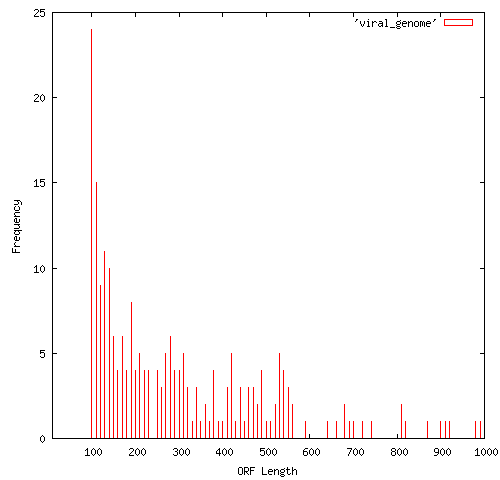
\includegraphics[scale=0.5]{viral_genome.png}
\caption{Histogram of Viral Genome ORF length v/s Frequencies}\label{fig:fs}
\end{figure}

\clearpage

The histogram for the ORFs in bacterial genomes is below. Contrast the histogram with the histogram of human genomic data. While the peak of this histogram is smaller, but the number of ORFs of lengths in the region 300-700 are significant as compared to human genome, where it steeply drops to nearly zero in that range.
\begin{figure}[htp]
\centering
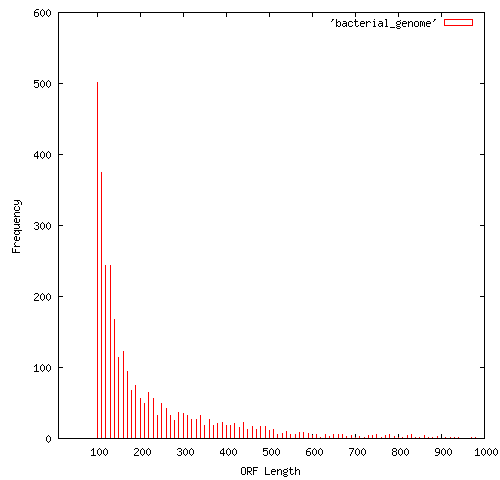
\includegraphics[scale=0.4]{bacterial_genome.png}
\caption{Histogram of Bacterial Genome ORF length v/s Frequencies}\label{fig:fs}
\end{figure}


The histogram below shows a distinct difference from viral and bacterial genomes. There are fewer ORFs of lengths longer than 300, but more ORFs of around 100-150 codons.
\begin{figure}[htp]
\centering
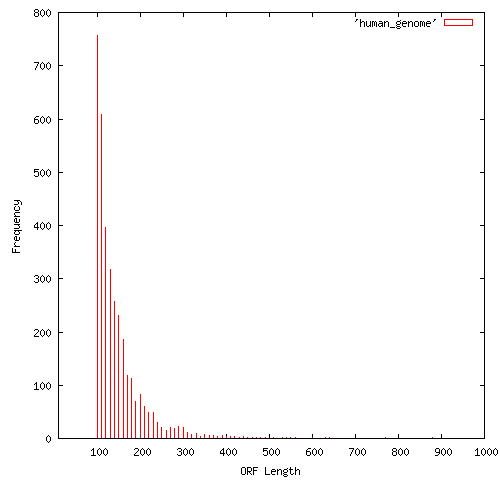
\includegraphics[scale=0.5]{human_genome.png}
\caption{Histogram of Human Genome ORF length v/s Frequencies}\label{fig:fs}
\end{figure}
\clearpage
The histogram below is for a Random DNA sequence, which was about the same size as the human and bacterial genome data. However, a clear distinction is that there are no ORFs of length more than 250 codons, and the number of ORFs with length greater than 100 decreases extremely steeply. This is inline with our expectations.

\begin{figure}[htp]
\centering
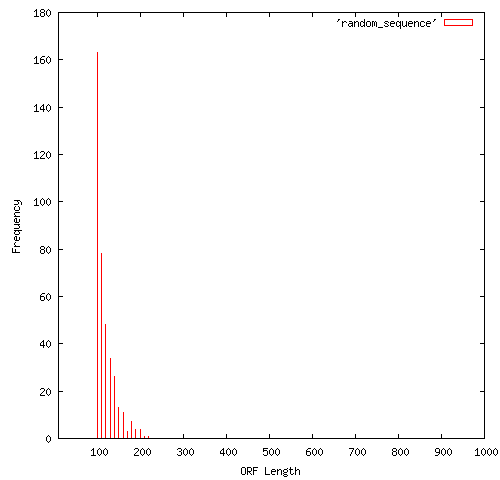
\includegraphics[scale=0.5]{random_sequence.png}
\caption{Histogram of Random DNA sequence ORF length v/s Frequencies}\label{fig:fs}
\end{figure}


\clearpage

\lstinputlisting[label=samplecode,caption=Source Code for the Open Reading Frames problem]{problem3.py}
\clearpage

 
\clearpage

\section{Shortest non-contiguous supersequence of two strings Problem}
This problem is solved using Dynamic Programming. Let $n$ and $m$ be the lengths of the two strings, $a$ and $b$ respectively, and $i$ and $j$ be the pointers in the strings. The problem is to find the shortest non-contiguous super-sequence of the two strings from $(i..n-1)$ and $(j..m-1)$. This problem can be solved by solving its sub-problems of getting super-sequences for smaller strings:
\begin{enumerate}
\item If $a[i]$ == $b[j]$, then both the characters overlap in the super-sequence, and the length of the supersequence is 1 + length of shortest non-contiguous super-sequnce for the two strings from $(i+1..n-1)$ and $(j+1..m-1)$
\item The character $a[i]$ is in the supersequence, and the length of the supersequence is 1 + length of shortest non-contiguous super-sequnce for the two strings from $(i+1..n-1)$ and $(j..m-1)$
\item The character $b[j]$ is in the supersequence, and the length of the supersequence is 1 + length of shortest non-contiguous super-sequnce for the two strings from $(i..n-1)$ and $(j+1..m-1)$
\end{enumerate}

If $i = n-1$, and $j < m-1$, then all the remaining characters in $b$ would be inserted in the super-sequence. Similarly, if $j = m-1$, and $i < n-1$, then all the remaining characters in $a$ would be inserted in the super-sequence.
\\
Thus, the DP table is $n$x$n$, and hence the space complexity is $O(n^2)$. Since, there are $n^2$ cells, one for each problem, and we can solve it using the results of its sub-problems in constant time, filling each cell requires constant time. Overall, filling the DP table requires $O(n^2)$ time. 

The code for the solution is as follows:
\lstinputlisting[label=samplecode,caption=Dynamic Programming solution for the problem]{problem_4_snippet.cpp}
\clearpage

\section{Minimum Length Palindrome Problem}
This problem is solved using Dynamic Programming. Let $i$ and $j$ be the pointers to the starting position in the string and the ending position in the string. The problem is to find the minimum length palindrome of the string between $i$ and $j$. Now, if the characters, $str[i]$ and $str[j]$ don't match, we have two options:
\begin{enumerate} 
\item Insert the character $str[i]$ before the position $j$, at the cost of one character, and solve the problem for the string between $i+1$ and $j$.
\item Insert the character $str[j]$ before the position $i$, at the cost of one character, and solve the problem for the string between $i$ and $j+1$.
\end{enumerate}
If $str[i]$ and $str[j]$ match, we simply solve the sub-problem for the string between $i+1$ and $j-1$.
The cost of solving the smallest sub-problem problem for the string between $i$ and $i$, is obviously 0, since the string has only one character in it. Thus, the DP table is $n$x$n$, and hence the space complexity is $O(n^2)$. Since, there are $n^2$ cells, one for each problem, and we can solve it using the results of its sub-problems in constant time, filling each cell requires constant time. Overall, filling the DP table requires $O(n^2)$ time. 

The code for the solution is as follows:
\lstinputlisting[label=samplecode,caption=Dynamic Programming solution for the problem]{problem_5_snippet.cpp}
\clearpage

\section{Pizza Picking Problem}
In this problem, we again use the Dynamic Programming approach. The constraint of the problem is such, that at any given time the gaps in the pizza pie would be contiguous. If there are $n$ slices in the pizza, picking any slice as the pivot, we start numbering each slice from $0$ to $n-1$ in clockwise order. Now, when Alice and Bob start picking slices, there would be only one contiguous gap in the pizza pie. This gap can be described by two indices, $i$ and $j$, the first missing slice and the last missing slice, in clockwise order. We solve the problem from Alice's perspective, and hence when we have a pizza with a contiguous gap from $i$ and $j$, the problem is to maximize the total area of pizza slices that Alice gets.

If we know $i$, $j$ and whose turn it is to take the next slice, we move ahead by taking a pizza from either of the ends, adding the slice area to alice's account if it was alice's turn, and then solving the subproblem of picking slices from the remaining pizza, and allowing the other person to pick a slice this time. In Alice's turn, Alice chooses the slice which maximizes the result, whereas in Bob's turn, Bob chooses the slice, which minimizes the result (remember, the result is the maximum area of the pizza that Alice consumes, so Bob, playing optimally, would obviously try to minimize this). 

Hence the state of the Dynamic Programming solution is $i$, $j$, and $turn$. $turn$ is 1, when its Alice's turn to pick a slice, and 0 when its not. Thus the DP table would be of size $n.n.2$, which is $O(n^2)$ space complexity. From one problem, we can reach to a sub-problem in constant time, and thus each cell in the table would be filled in constant time. Since there are at most $n^2$ cells in the DP, it takes $O(n^2)$ time.

The code for the solution is as follows:
\lstinputlisting[label=samplecode,caption=Dynamic Programming solution for the problem]{problem_6_snippet.cpp}

There exists, another elegant solution which does not require the $turn$ variable in the DP state.

\end{document}
